\chapter{Phase 2: System Interaktion und Bedienung}

\section{User Stories}

Nun werden die Usecases aus Phase 1 mithilfe von User Stories weiter beschrieben. Dabei liegt der Fokus auf Szenarien, die eine Interaktion mit dem Smartwatch-System abbilden.
Die ersten beiden User Stories beschreiben zunächst einen typischen Hauptanwendungsfall der Uhr: Das Annehmen/Ablehnen/Tätigen von Anrufen von dem verbundenen Smartphone.
Um dem Produkt eine detailgetreue Anleitung für einen reibungslosen Einrichtungsprozess beizulegen, wurde eine User Story speziell für das Einrichten, bzw. Koppeln der Smartwatch mit einem Smartphone definiert.
Da eine Kernfunktionion der Smartwatch darin besteht, sie für Fitness-Tracking verschiedener sportlichen Aktivitäten einzusetzen, wurden mehrere User Stories für diese Anwendungsfälle entworfen. Im folgenden wird die User Story "Joggen gehen" beschrieben, weitere Fitness-User Stories finden sich im Anhang an diese Arbeit.
\begin{figure}[H]
\centering\
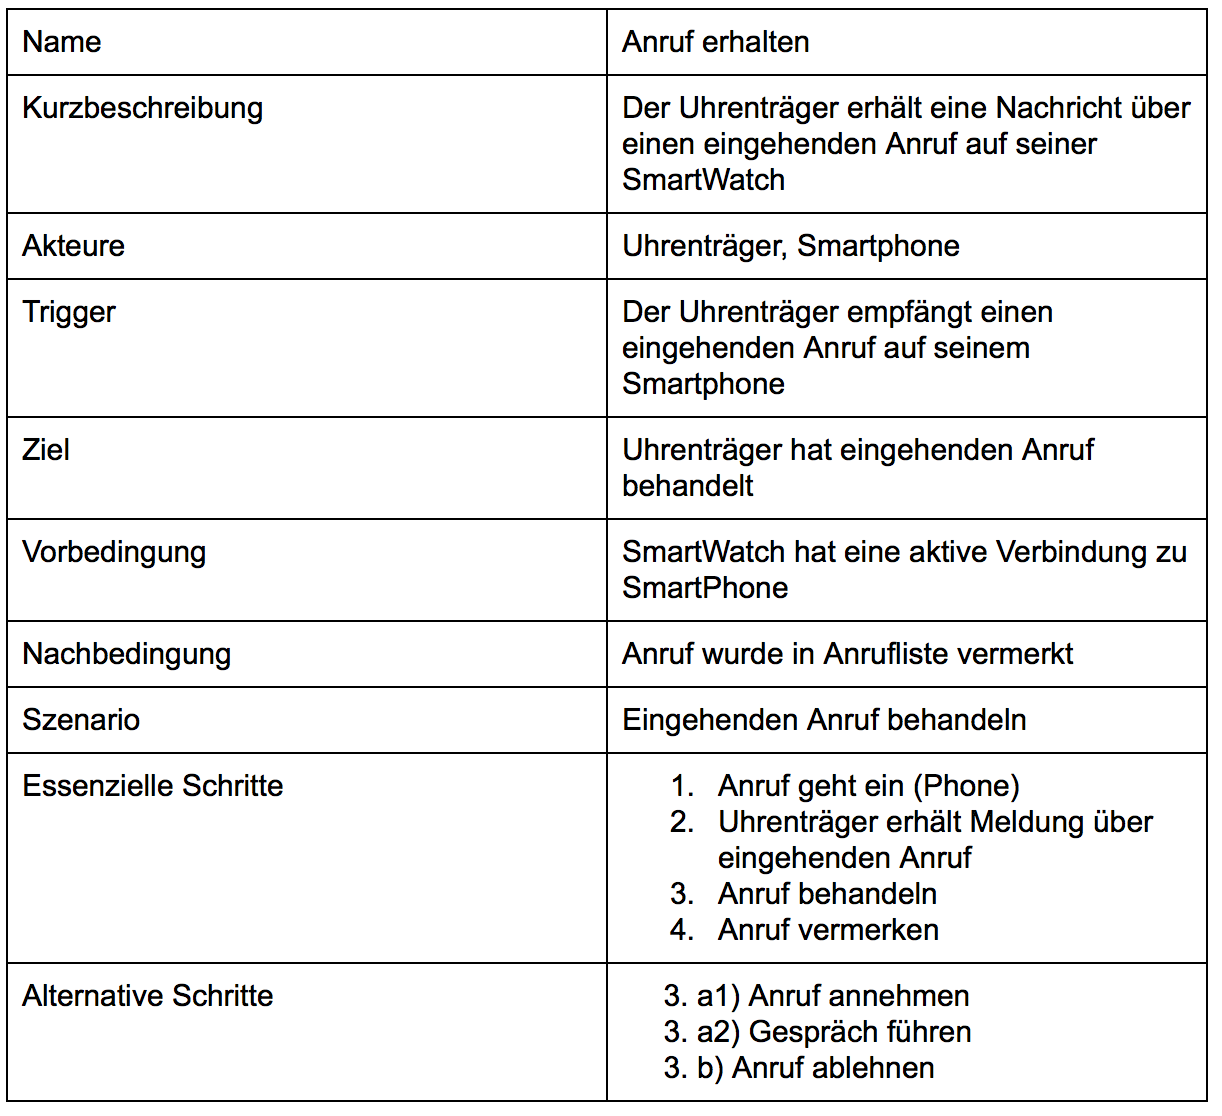
\includegraphics[width=10cm]{img/story_in}
\caption{User Story - Eingehender Anruf}\label{fig:story-in}
\end{figure}
\begin{figure}[H]
\centering\
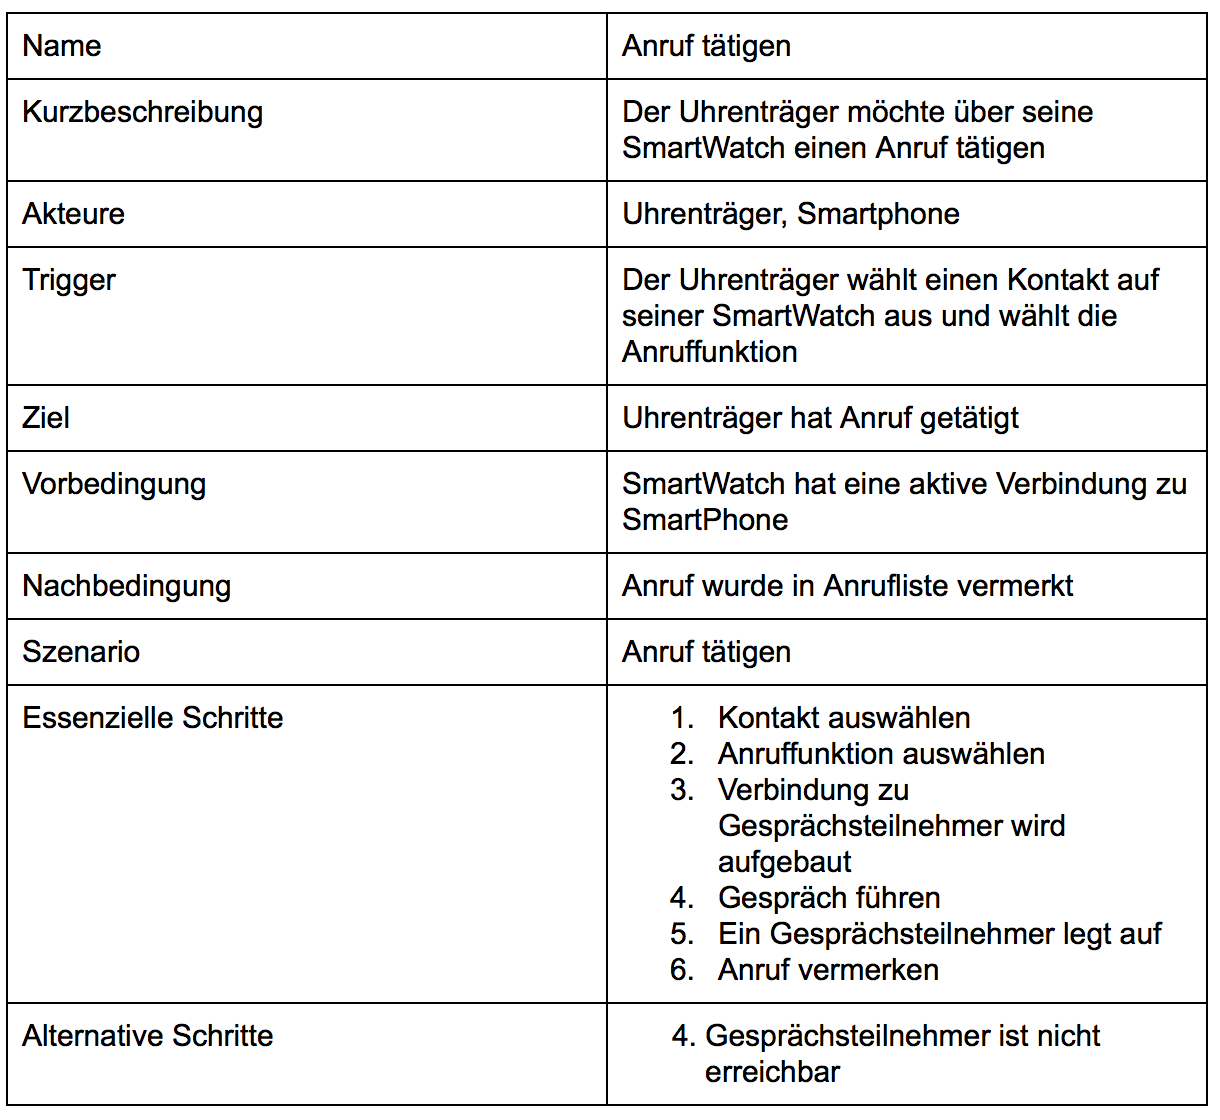
\includegraphics[width=10cm]{img/story_out}
\caption{User Story - Anruf tätigen}\label{fig:story-out}
\end{figure}
\begin{figure}[H]
\centering\
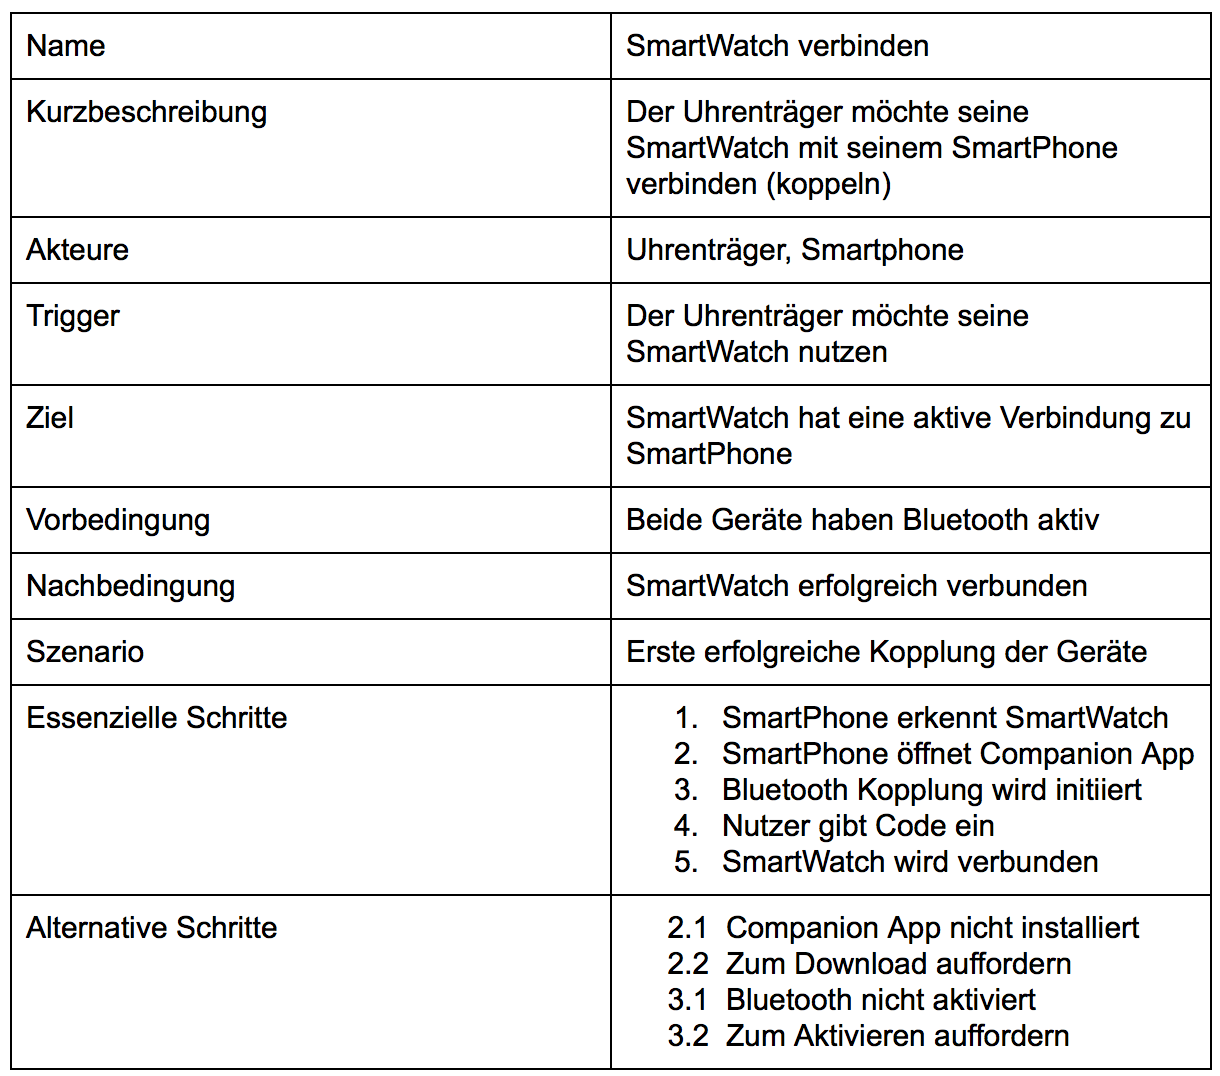
\includegraphics[width=10cm]{img/story_pairing}
\caption{User Story - Pairing}\label{fig:story-pairing}
\end{figure}
\begin{figure}[H]
\centering\
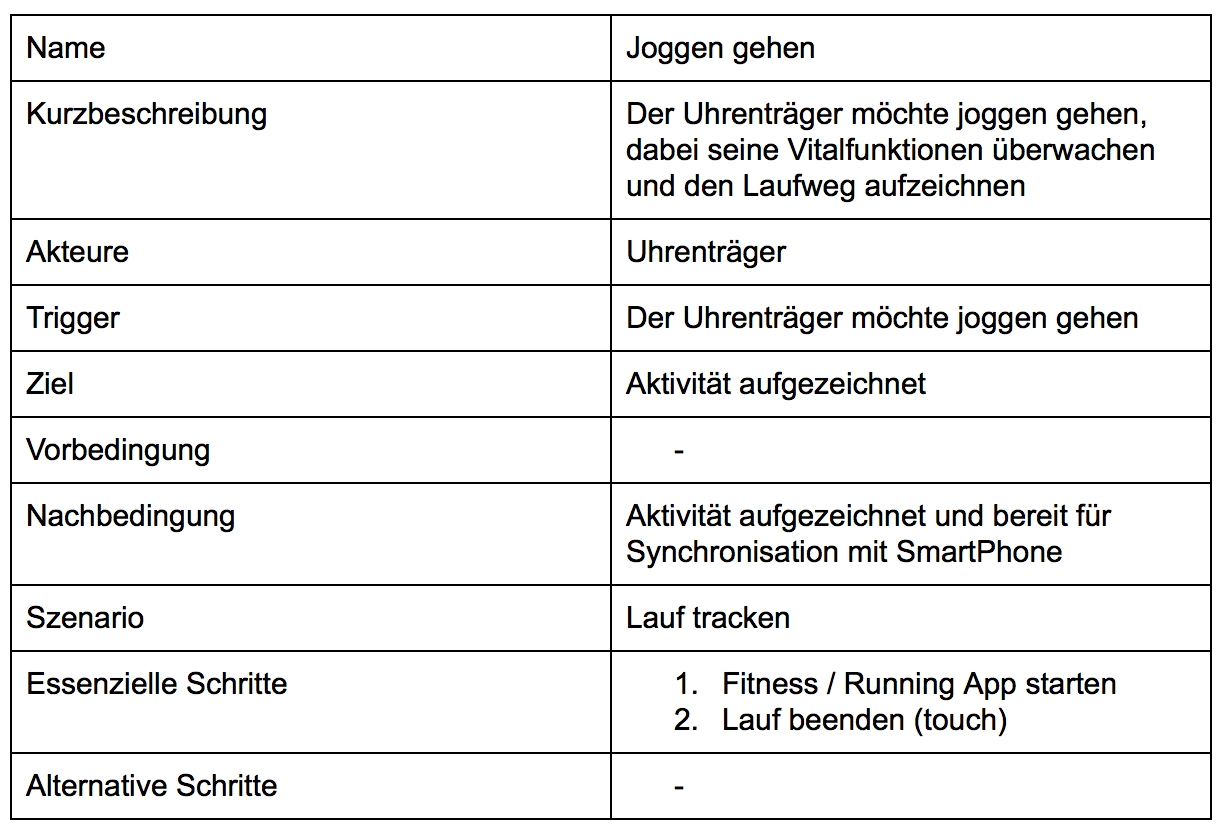
\includegraphics[width=10cm]{img/story_joggen}
\caption{User Story - Fitness}\label{fig:story-joggen}
\end{figure}

\section{Sequence Diagram}
Das Interaktionsverhalten für die Szenarien Anruf und Koppeln des Smartwatches mit dem Smartphone, ist fest definiert. Sequenzdiagramme eignen sich zur Kontextabgrenzung sehr gut.\\
In der ~\ref{fig:kopplung} ist der Bluetooth-Kopplungsvorgang als Sequnzdiagramm abgebildet.
Zuerst startet der Smartphone über Bluetooth eine Discovery-Anfrage in der Umgebung.
Das Bluetooth des Smartphones sucht alle verfügbaren Bluetooth-Geräte in der Nähe und übergibt diese dem Smartphone für die Anzeige.
Der Benutzer kann seinen Smartwatch in der Liste auswählen um die Kopplung zu starten.
Danach wird der Benutzer aufgefordert auf seinem Smartphone jetzt die Bluetooth-Kopplungsanforderung mit dem Kopplungs-Code zu bestätigen. Der Kopplungs-Code wird in der Smartwatch angezeigt.
Falls der Benutzer einen falschen Code eingeben hat, wird die Kopplung vom Smartwatch 
abgelehnt.

\begin{figure}[H]
\centering\
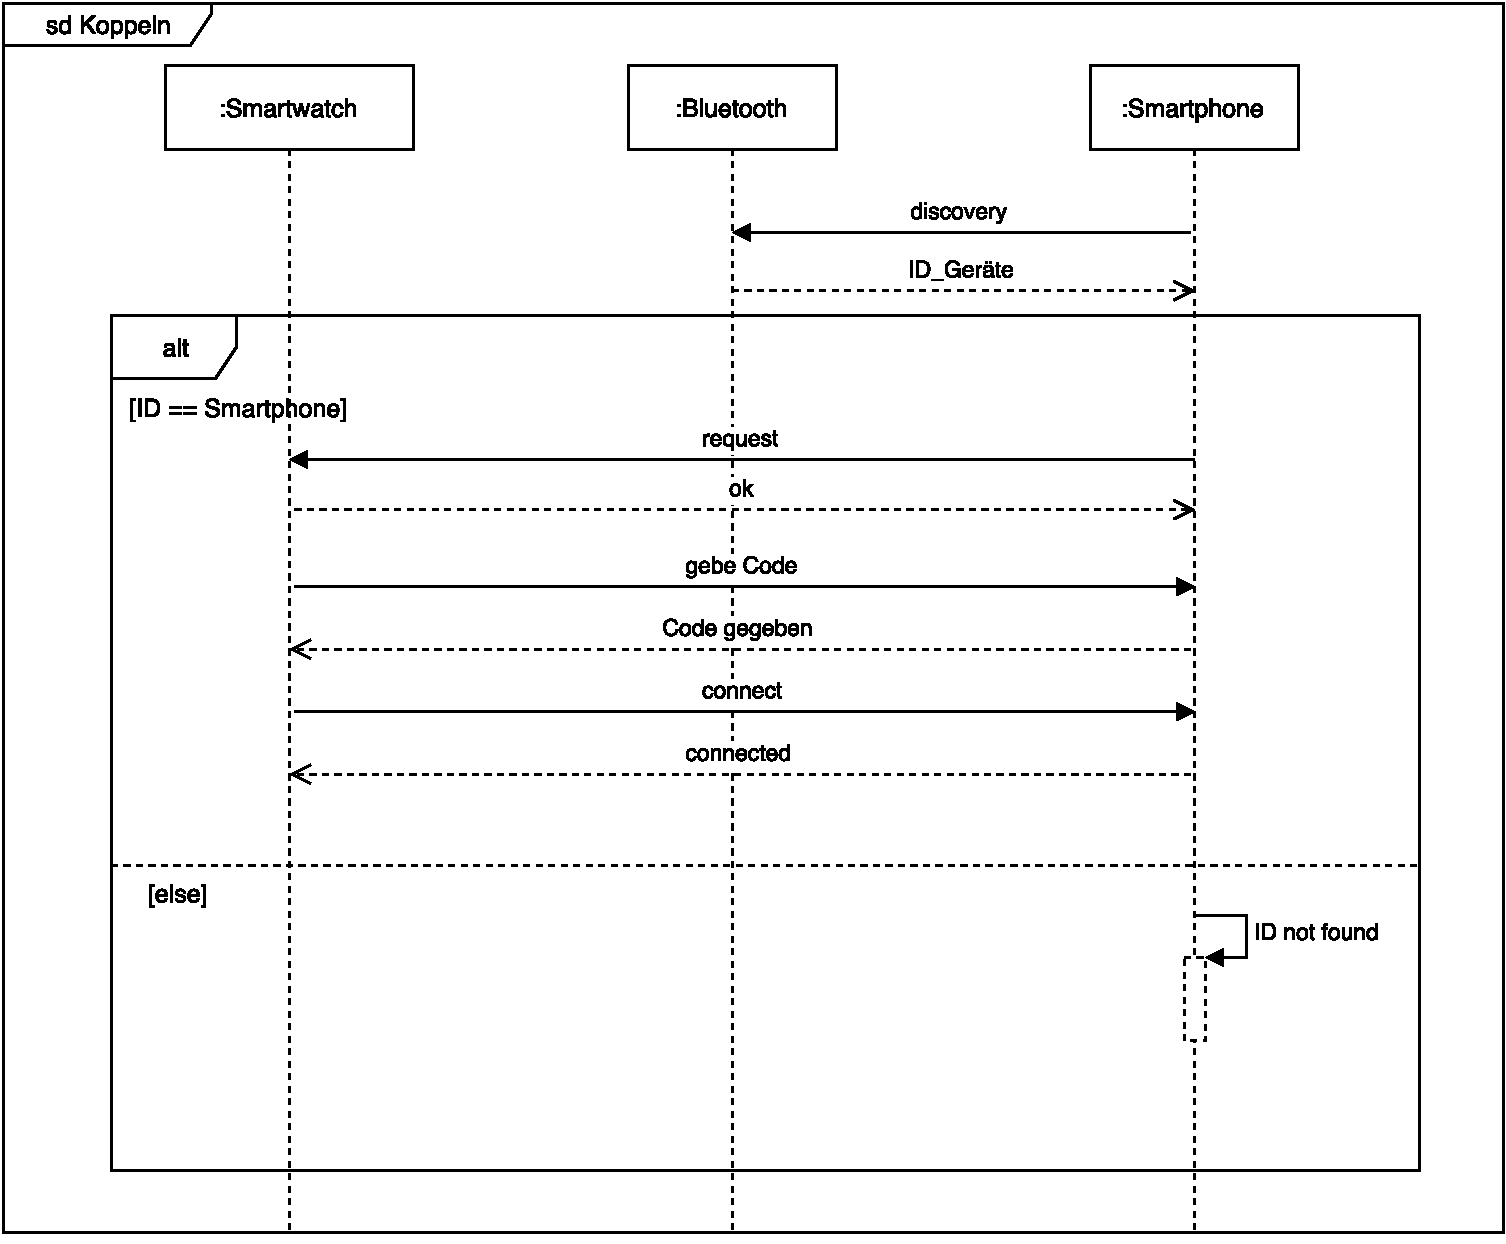
\includegraphics[width=10cm]{img/KoppelnSequenz}
\caption{Kopplung des Smartphones mit Smartwatch}\label{fig:kopplung}
\end{figure}






\section{State Diagram}

\section{Timing Diagram}

